Although this is called the intro, I've also but int bits that I want to put in that are general for more than one chapter. These need to be sorted eventually...

\section{Statistical Ecology}

Some general remarks about stat ecol perhaps.

\section{Themes}

\bi
	\item Morphing
	\item Modifying penalties
	\item Computational efficiency
	\item Realistic physical models!!!!!!
\ei


\section{Some notational conventions}



\section{Generalized Additive Models}

General GAM setup

\bi
\item Splines
\item objective function
\label{GAMobjfcn}
\item penalties
\item bases - TPRS and maybe P-splines?
\item fitting - GCV REML etc
\item other stuff
	\bi
	\item MSE
	\begin{equation}
\text{MSE}(\hat{f}) = \frac{1}{P} \sum_{j=1}^P (\hat{f}(x_j) - z_j)^2,
\end{equation}
the mean difference between the model ($\hat{f}$) evaluated at the prediction points ($\{x_j : j=1 \dots P\}$) and the true value of the function ($\{z_j : j=1 \dots P\}$.) This gives the MSE per model, since here many realisations are run, the mean of these over all simulations is taken and the standard error is calculated.
	\item EDF
	The estimated degrees of freedom of a model gives an idea of the complexity of the spline that was fit to the data, the higher the EDF, the more basis functions were used and  the more complex the model.  Since the models used here are penalised, it is the penalty term that controls the overall ``wigglyness'' of the spline and hence the EDF. Although the basis dimension is set in the model this is just an upper bound, the smoothing penalty suppresses parts of the model. Therefore basis dimension is not a major concern provided that it is not set too low (\cite{simonbook}, p. 161.) 

	\ei
\ei

\section{Finite area smoothing}

\subsection{Overview of finite area smoothing}

Splines are a popular way of performing spatial smoothing in two dimensions. In this context, they are used to fit smooth functions over a geographical region. A typical application of this is in ecological modelling; a response is sought (be it the density of a population or concentration of a chemical) as a function of its spatial coordinates. The function can then be used to perform inference on the population, whether that be an abundance estimate, density map or a more sophisticated inferential goal.

% leakage example 
\begin{figure}
\centering
% trim order l b r t
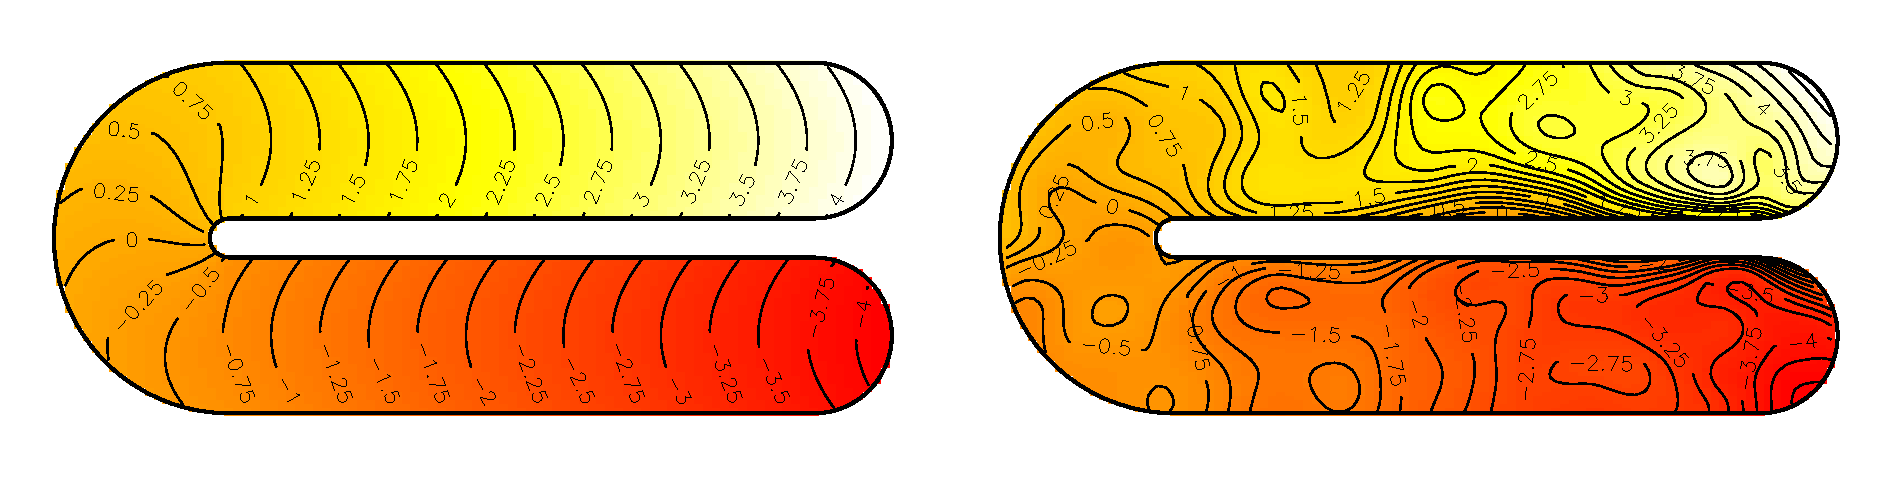
\includegraphics[width=4in]{intro/figs/ramsay-leak.pdf}\\
\caption{An example of leakage. A thin plate regression spline was fit to data sampled from the function on the left, here the model smooths across the gap in the middle of the domain (right.)}
\label{leakage}
\end{figure}

When the geographical region has a \emph{complex boundary}, features from one part of the domain can unduly influence other parts. Typically a complex boundary consists of having some peninsula-like feature(s) in the domain with notably different observation values on either side of the feature; there must also be some scientific motivation as to why those parts of the domain should not affect each other. Features such as peninsulae give rise to a phenomenon known as \emph{leakage}; a typical example can be seen in \fig{leakage}. Leakage is problematic since it causes the fitted surface to be mis-estimated; this can then lead to incorrect inference (eg. incorrect abundance estimates), which is clearly not desirable. This can be seen in \fig{leakage} where the high values in the upper part of the domain leak across the gap to the lower values below and vice versa.

\subsection{Ramsay's horseshoe function as a benchmark for finite area smoothing}

\cite{ramsay} proposes a function which can be used to benchmark new approaches to 2-dimensional smoothing. The function takes the form of a horseshoe which is flat across the domain but ranges from $-4$ to $4$ along the domain's major axis. \cite{soap} modifies the shape by adding curvature across the minor axis of the shape. The so-called ``Ramsay horseshoe'' is shown in \fig{leakage}.

The test function highlights a common problem in spatial smoothing: that of ``leakage''. When the problem is specified in Euclidean distance, the model thinks that the distance between the $-4$ and $4$ points of the horseshoe is the distance over the gap in between them, rather than the distance along the major axis of the shape. This causes the high density from one side to contaminate the other (or the low to contaminate the high.) It is easy to see that this causes the smooth to be calculated incorrectly.


It differs from the figure in \cite{ramsay} in that a slight curvature in the function along the major axis has been added such that the gradient is not perpendicular to the boundary. This curvature was added in \cite{soap}  in order to avoid the horseshoe function lying in the nullspace of the soap film's penalty, making the problem too easy for a soap film smoother.
		

\subsection{Previous approaches}

The cause of leakage can be characterised in two ways: either the smooth does not respect the boundary of the domain, or the smooth does not take into account the geometry of the domain; in particular with regard to the distance between points within the domain. Previous work in this area has been to combat leakage along these two lines. Work of \cite{ramsay} and \cite{soap} both use a PDE boundary condition approach to try to prevent leakage, where as \cite{wangranalli} and \cite{eilerstalk}  attempt to approximate the intrinsic structure of the domain while not treating the boundary a something special in the basis setup. Here I will be adopting the the latter approach.

The four main works on the topic may be summarised as follows:

\begin{enumerate}
\item \cite{ramsay} proposes finite element $L$-splines (FELSPLINEs.) The $L$-spline has a differential operator in its penalty, which cannot be analytically solved in two dimensions. However, to combat this, the author triangulates the domain and then constructs a set of bivariate quadratic polynomial basis functions over each triangle, specifying that there be continuity over the edges of the triangles. The union of these functions is then a solution to the PDE in the penalty and therefore the solution to the usual smoothing objective function (see \secref{GAMobjfcn}.)

Although FELSPLINE does not exhibit leakage on the horseshoe, in practice it make unrealistic assumptions about the model it fits. The boundary conditions of FELSPLINE specify that the gradient is normal to the boundary at every point, this is not always physically realistic and as \cite{soap} showed, merely by adding a small amount of curvature to the gradient of the Ramsay horseshoe, the method's performance begins to falter.

\item \cite{wangranalli} adopt a ``within-area distance'' formulation for thin plate splines. In this case they take the geodesic distance between two points, that being the shortest path within the domain. This gives a definition of how near objects are in the domain.

Since the geodesic distance is only known if the intrinsic structure of the domain is known (which is rare in ecological examples), the authors use a different method to calculate the shortest path. For this they create a graph, with datum at each node and the distance between each pair of nodes as the weights on the edges. Floyd's algorithm\footnote{Which is cubic in the number of vertices.} is then used to find the $k$ nearest neighbors of each node.


\item \cite{soap} consider constructing a soap film over the domain. The film is then weighed down by the data, the objective is then to minimize the surface tension in the film.

\item An alternative approach is to ``morph'' the area in question to be one which is more suitable for smoothing. For example, with Ramsay's horseshoe, it seems intuitive to simply bend the horseshoe into a long strip and then smooth on that domain. This is what we propose here. 

This approach raises some questions. First, what is the natural domain to transform to? Second, what is the nullspace of the penalty term of a spline in this new domain? Clearly for some shapes the answer to both of these questions is obvious, but this is not always the case. We address these problems below.


\end{enumerate}


\bi
\item Comparison of different approaches
	\bi
		\item p. 2 of ramsay writeup for \sch
		\item MDS report intro
		\item Want to summarise each of the papers.
	\ei
\ei

\section{Distance sampling}


